\chapter{Asking Beverly Hills Billionaires How They Got So RICH!}

These notes follow a School of Hard Knocks field lecture, with chapter curation by LazyingArt LLC, and they should be read with one caution in mind from the start: this lecture gives us almost no reliable board-work or slide-work to read from, so every equation below is reconstructed from the spoken record. The host begins with spectacle, but he does so deliberately. We are shown a Rolls-Royce, a mafia reveal, and a corporate-celebrity reveal before the inquiry is stated in plain language. Only then are we told the real problem: in Beverly Hills, what operating grammar produced the visible wealth?

\section{Cold Open: Beverly Hills as Search Problem}

We begin, then, not with a doctrine but with a baited montage. The visible object comes first and the explanation comes second. This is not accidental. The lecture wants us to feel the pull of the outcome before it asks us to reverse the causal arrow and reconstruct the machine beneath it.

Once the host states the mission, the episode becomes more disciplined. He is cold-approaching multi-millionaires and billionaires in Beverly Hills to ask not merely \emph{who} is rich, but \emph{how} the fortune was built. That distinction is the real opening move. A luxury car, a celebrity title, or a startling biography is treated as data; the chapter that follows is the attempt to infer the mechanism.

It is useful to mark the mechanism-bank explicitly at the outset, because the lecture itself keeps shifting the position in the machine under inspection.

\begin{table}
\centering
\begin{tabular}{p{3.1cm}p{3.2cm}p{2.6cm}p{4.5cm}}
\hline
Case & Position in the machine & Key number & Core mechanism \\
\hline
Gel-nails founder & inventor and distributor & \(\$25\) price, \(\$1\) cost & extreme unit margin, retained profit, global expansion \\
Oil-and-gas operator & dealmaker & revenue stated as \(>\$10\) million and \(<\$100\) million & transfer capture, persistence, relationships \\
Former mafia operator & organizer and negotiator & \(5\times 10^8\) gallons/month & delegation, leverage, large-scale extraction \\
Plastic surgeon from Ghana & high-income professional turning owner & \(\$9\) million/year & diversification from practice income into industrial asset ownership \\
Chipotle CEO & scaled executive and operator & \(\$13\) billion sales, \(>3800\) stores & controlled growth, fortress balance sheet, accountability \\
\hline
\end{tabular}
\caption{Transcript-derived mechanism map. The lecture does not repeat one generic success formula; it moves across several distinct wealth positions.}
\end{table}

That table is not the lecture itself. It is only a map. The lecture insists on a narrative order, and we should preserve it: invention first, then intermediation, then harder forms of leverage, then the host's own access business, then professional income turning toward industrial scale, and finally the most orderly corporate example.

\section{Invention, Margin, and Reinvestment}

The first full case is the gel-nails founder, and the lecture gives us its first clean piece of arithmetic almost immediately. We hear that he invented gel nails in 1981, began with only \(\$200\) on Venice Beach, never borrowed money, and scaled by putting profit back into the business. The numerical core is unusually sharp for this series, so it deserves to be written cleanly.

\begin{definition}
By \emph{unit economics} we mean the arithmetic attached to one unit of output: selling price, direct cost, unit profit, and gross margin. The lecture's first serious wealth mechanism is expressed at exactly this level.
\end{definition}

The spoken numbers are:
\begin{align}
P_{\mathrm{gel}} &= \$25, &
C_{\mathrm{gel}} &= \$1, \\
\pi_{\mathrm{gel}} &= P_{\mathrm{gel}}-C_{\mathrm{gel}}=\$24, &
m_{\mathrm{gel}} &= \frac{\pi_{\mathrm{gel}}}{P_{\mathrm{gel}}}
= \frac{24}{25}\approx 0.96 .
\end{align}

This is the first moment where the lecture becomes mathematically explanatory rather than merely anecdotal. A \(96\%\) gross margin is not scale by itself, but it changes the financing problem. Once that number is in place, the later claim that there was no line of credit, no mortgage, and no borrowing for forty-four years no longer sounds like mythology. It sounds like a business with unusually powerful self-financing capacity.

We can formalize the reinvestment mechanism with the mildest possible notation:
\begin{equation}
K_{t+1}=K_t+\Pi_t-W_t,
\end{equation}
where \(K_t\) is retained business capital after stage \(t\), \(\Pi_t\) is operating profit during that stage, and \(W_t\) is owner withdrawal. We use \(W_t\) here rather than \(D_t\) so that later \(D\) may remain available for debt.

The initial condition is tiny:
\begin{equation}
K_0 \approx \$200.
\end{equation}

The lecture does not hand us an overhead model, but it gives enough structure for a stripped-down worked example. If \(n\) units are sold, then at the level of direct contribution we have
\begin{align}
\Pi(n) &= 24n, \\
K_1 &= K_0 + \Pi(n) - W_0 = 200 + 24n - W_0 .
\end{align}
For instance,
\begin{equation}
\Pi(10^4)=24\times 10^4=\$240{,}000.
\end{equation}
This is not a full income statement. It is only an explanatory skeleton. But it tells us why the lecture places margin before it places scale.

The lecture then immediately widens the mechanism. The founder is not just an inventor. He says product \emph{and} distribution matter. He is in \(90\) countries:
\begin{equation}
N_{\mathrm{countries}}=90.
\end{equation}
And he says, in effect, that globalization was the play already in the 1980s. So we should not mistakenly reduce the story to invention alone. The loop is invention, margin, retained profit, distribution, and then enlarged market reach.

\begin{figure}
\centering
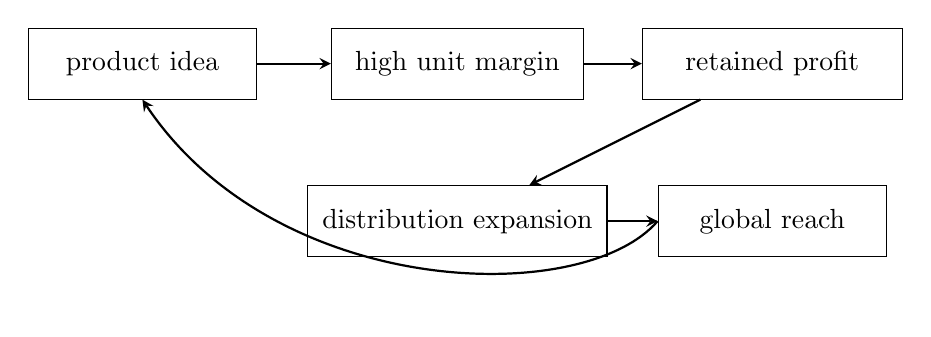
\begin{tikzpicture}[>=stealth]
\node[draw, rectangle, minimum width=2.9cm, minimum height=0.9cm] (a) at (0,0) {product idea};
\node[draw, rectangle, minimum width=3.2cm, minimum height=0.9cm] (b) at (4,0) {high unit margin};
\node[draw, rectangle, minimum width=3.3cm, minimum height=0.9cm] (c) at (8,0) {retained profit};
\node[draw, rectangle, minimum width=3.8cm, minimum height=0.9cm] (d) at (4,-2) {distribution expansion};
\node[draw, rectangle, minimum width=2.9cm, minimum height=0.9cm] (e) at (8,-2) {global reach};

\draw[->, thick] (a) -- (b);
\draw[->, thick] (b) -- (c);
\draw[->, thick] (c) -- (d);
\draw[->, thick] (d) -- (e);
\draw[->, thick] (e.west) .. controls (5.6,-3.1) and (1.7,-3.0) .. (a.south);
\end{tikzpicture}
\caption{Transcript-derived schematic of the first case. The lecture treats invention, margin, reinvestment, and distribution as one loop rather than as separate topics.}
\end{figure}

The founder then adds two further notes, and both matter. First, the origin story is engineering and transfer: he says he used a gel from dental work and moved the idea from teeth to hands. Second, he insists on sales. The inventor is not protected from commerce. ``You have to sell yourself first'' is part of the mechanism, not an ornamental motivational line.

The case closes with an anti-consumption contrast. The visible Rolls-Royce remains in the frame, but the point becomes the refusal to spend list price. The direct arithmetic is:
\begin{equation}
P_{\mathrm{car,list}} \approx \$520{,}000, \qquad
P_{\mathrm{car,auction}} \approx \$175{,}000, \qquad
\Delta P \approx \$345{,}000.
\end{equation}
We retain this direct interview arithmetic and do not merge it with the host's later paraphrase, which inflates the affordability claim. The deeper point is that capital is not to be confused with costume.

\subsection{Question \& Answer}

\paragraph{Question.} How do we scale to nine figures without borrowing money?

\paragraph{Answer.} The lecture's answer is local rather than universal. We begin with unusually favorable unit economics, we keep withdrawals modest relative to profit, and we iterate
\[
K_{t+1}=K_t+\Pi_t-W_t.
\]
If margin is high enough and profits are repeatedly fed back into the business, retained capital can finance further distribution and further growth. The speaker is not claiming that debt is always unnecessary. He is showing that in this particular business the margin was strong enough to let reinvestment do the compounding work.

At the end of the segment the host gives his own interpretive recap, and that recap is worth preserving. He says, in effect, that the interview should not be read as permission to buy the car. It should be read as a lesson in saving, anti-waste, and empire-building. Even here, however, the lecture is careful not to collapse everything into thrift alone. The founder also says he failed several times before the big success and invokes the logic of repeated swings. So the full mechanism is not mere restraint; it is restraint joined to invention and repeated attempts.

\section{Intermediation and Transfer Capture}

The next case changes the position in the machine. We move away from the inventor and toward the dealmaker. The oil-and-gas operator says he is not the land man; he is the one who puts the deals together. This is the first explicit turn toward intermediation.

The lecture's own phrasing suggests a clean schematic:
\begin{equation}
\mathcal I
=
\text{resource owner}
\longleftrightarrow
\text{dealmaker}
\longleftrightarrow
\text{capital / operator}.
\end{equation}
The important point is that the middle term is not mere commentary. If a transaction cannot be completed without search, trust, assembly, or negotiation, then the middle node can become a source of wealth in its own right.

\begin{figure}
\centering
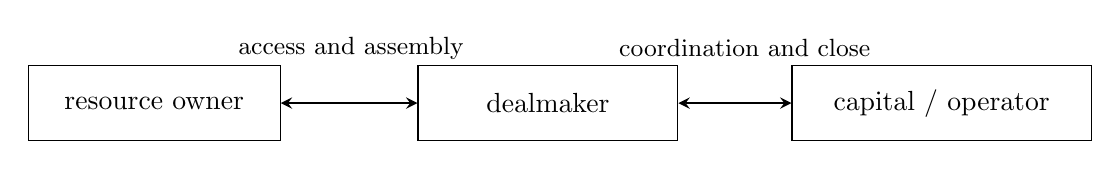
\begin{tikzpicture}[>=stealth]
\node[draw, rectangle, minimum width=3.2cm, minimum height=0.95cm] (o) at (0,0) {resource owner};
\node[draw, rectangle, minimum width=3.3cm, minimum height=0.95cm] (m) at (5,0) {dealmaker};
\node[draw, rectangle, minimum width=3.8cm, minimum height=0.95cm] (p) at (10,0) {capital / operator};

\draw[<->, thick] (o) -- (m);
\draw[<->, thick] (m) -- (p);

\node at (2.5,0.7) {\small access and assembly};
\node at (7.5,0.7) {\small coordination and close};
\end{tikzpicture}
\caption{Transcript-derived wealth-transfer junction. The lecture's claim is that the transfer point itself may become the lucrative position.}
\end{figure}

The host sharpens the point with a line he attributes to a prior Wall Street interview: when wealth moves from one person to another, someone in the middle transfers it, and that person also becomes wealthy. The oil-and-gas speaker does not produce a theory in reply. He simply concedes that one can look at it that way. That small concession is enough. The lecture is not proving a theorem of markets; it is identifying a repeatable occupational geometry.

We should also keep the biography attached to the mechanism. The speaker came from nothing, calls himself a high-school dropout, and says that relationships were decisive in entering the business. Some work rewards what one knows; some work rewards who one knows. In this case the field is entered through relationship and then defended through persistence.

\subsection{Question \& Answer}

\paragraph{Question.} Why does the middleman so often become wealthy?

\paragraph{Answer.} Because the middle position can sit at a necessary transfer junction. If owner and operator cannot transact directly without assembly or trust-building, then the coordinating agent can charge for making the transfer happen. In the lecture's terms, wealth is not captured only at the source of the asset or at the final site of operation. It may also be captured at the point where the transaction becomes possible:
\[
\text{owner}\longleftrightarrow \text{dealmaker}\longleftrightarrow \text{operator}.
\]

The host then asks for sales and negotiation advice, and the answer is almost crude in its simplicity: do not take no for an answer. We should not dismiss that as empty bravado. In this case persistence is the behavioral correlate of the intermediation diagram. If the middle position lives on repeated attempts to assemble difficult deals, then refusal-saturation is part of the operating method.

There is one more useful detail in the segment. The oil-and-gas speaker gives a money ethic quite different from the earlier founder's frugality ethic. He says not to be afraid to spend money and that one will always make more. The lecture is already telling us that there is no single universal doctrine of money-management here. The inventor emphasizes saving; the dealmaker emphasizes forward motion and appetite. The chapter should keep that tension visible.

\section{Delegation, Negotiation, and Accountability Under Pressure}

The next interview intensifies the same transfer logic into a criminal extreme. We should resist the temptation to turn it into sensationalism alone. The lecture uses this case to extract several unusually sharp mechanisms: scale, delegation, leverage, leadership, etiquette under pressure, and accountability.

The numerical claim is large enough that it must be treated cautiously and explicitly. The speaker says he was selling a half-billion gallons of gas a month and taking down thirty to forty cents a gallon:
\begin{equation}
q_{\mathrm{gas}}\approx 5\times 10^8\ \text{gallons/month}, \qquad
s_{\mathrm{gas}}\in[\$0.30,\$0.40]\ \text{per gallon}.
\end{equation}
If we multiply these directly, we obtain the implied monthly gross take
\begin{equation}
\Pi_{\mathrm{gross,month}}=q_{\mathrm{gas}}\,s_{\mathrm{gas}}
\approx \$1.5\times 10^8 \text{ to } \$2.0\times 10^8.
\end{equation}
At the same time, the speaker gives weekly figures that are much smaller:
\begin{align}
\Pi_{\mathrm{week}} &\in [\$8\times 10^6,\$15\times 10^6], \\
\Pi_{\mathrm{week,peak}} &\approx \$10\times 10^6 \text{ to } \$12\times 10^6 .
\end{align}

\begin{remark}
These quantities do not reconcile cleanly if treated as one consistent bookkeeping model. The correct move is not to repair them by guesswork. We preserve them as speaker-attributed scale claims and keep the mismatch visible.
\end{remark}

Once the numerical shock has done its work, the lecture pivots to organization. ``Do what you do best, delegate the rest'' is the speaker's operating rule. Here the machine enlarges because the leader no longer performs every function directly. He surrounds himself with the right people, motivates them to do the work he will not do, and becomes, in his own language, the mastermind or leader.

The lecture then distinguishes leader from boss in a way that is better than its setting might suggest. A boss can command. A leader is followed willingly. That matters because the section on Chipotle will later turn the same idea into a cleaner doctrine of accountability. Here it appears in rougher form: people stay when expectations are clear and when they are treated right.

The government-negotiation story then gives us the lecture's clearest instance of leverage. The speaker says he had beaten the government five times. They wanted him badly. Therefore he went into the negotiation with an edge. The structure is elementary but important: if the other side urgently wants something that only we can supply, bargaining power shifts. The lecture never turns this into symbolic game theory, and it should not be over-formalized; but the intuition is exact.

The prison material initially looks like a biographical side-channel, yet it serves the lecture's larger logic. In a high-friction environment where respect is unstable, small procedural words such as ``please,'' ``thank you,'' and ``excuse me'' are stabilizers. They are not merely niceties. They reduce the probability of escalation.

Accountability then reappears, but in personal rather than corporate form. The speaker says he was once accountable to an oath and to his boss, and is now accountable first to God and then to family. The point is not theological bookkeeping. It is that the object of accountability directs the path of action. The same mind can persist while the behavioral outcome changes because the governing authority has changed.

\subsection{Question \& Answer}

\paragraph{Question.} What do delegation and leverage actually buy a leader?

\paragraph{Answer.} Delegation enlarges the machine. It replaces one person's output with a coordinated set of specialized outputs. Leverage changes the negotiation boundary. If the other side needs our cooperation more urgently than we need theirs, the space of attainable outcomes shifts in our favor. The lecture presents these ideas through an extreme biography, but the structural lesson is general: scale requires organized work, and favorable negotiation requires an asymmetry in need.

The segment closes with a final rough lesson in determination. The speaker says, in different language, that nobody is coming to save you. This would be banal if it stood alone. But after the section's larger mechanics, it has a more definite meaning: no external authority substitutes for relentless movement through hard constraints.

\section{Interlude: Access Turned Into Product}

At this point the lecture interrupts itself. The host stops interviewing and turns the camera toward his own business. This interruption is structurally real and should remain visible, because it shows a second machine operating inside the first.

The arithmetic is straightforward:
\begin{equation}
F_{\mathrm{host}}\approx 12.7\times 10^6, \qquad
V_{\mathrm{month}}\approx 2\times 10^8, \qquad
N_{\mathrm{billionaires,US}}\approx 800, \qquad
N_{\mathrm{event}}=3.
\end{equation}
These are spoken marketing numbers, not independently verified operating statements, but the logic they support is clear. Attention is large, billionaires are scarce, the event count is small, and the offer is live-only. In other words, access itself is the product.

The lecture is careful to market not content in the abstract but \emph{proximity}: direct questions, live presence, no replay, no recording, limited window. This interlude is not the doctrinal center of the chapter, but it reveals that the interviewer is also a businessman selling a scarcity structure built from attention, curation, and gated access.

\section{From Professional Income to Industrial Ambition}

The Ghanaian plastic surgeon resets the tone. After invention, intermediation, and criminal leverage, the lecture now turns to professional labor at very high income and then asks whether even that is enough.

The first numerical anchor is direct:
\begin{equation}
Y_{\mathrm{surgeon}}\approx \$9\times 10^6 \ \text{in one year}.
\end{equation}
The segment begins not with industrial plans but with biography and domestic alignment. The worst financial decision, the speaker says, is marrying the wrong person. The transcript around faith and partnership is awkward in places, but the durable mechanism is plain enough: misalignment at home destroys attention, and a damaged attention field weakens creative and commercial output.

The lecture then binds this domestic argument to faith. Shared faith is treated as a proxy for aligned values, and aligned values are treated as protection against energy leakage. Whether or not one accepts the religious framing, the operational claim is intelligible: a disordered home front taxes productive concentration.

The next move is the important one. The speaker says that despite already knowing billionaires and earning very large sums, he is not yet at the scale he wants. The route to that larger scale is diversification:
\begin{equation}
W_{\mathrm{total}} = W_{\mathrm{practice}} + W_{\mathrm{industrial}}.
\end{equation}
The first term is the wealth generated by surgery practice. The second term is the wealth generated by ownership of a larger industrial asset. In the interview that second term is named explicitly as a pharmaceutical plant in Ghana, intended to be the largest in sub-Saharan Africa.

This is the lecture's cleanest statement that high professional income and billionaire-scale ownership are different objects. The speaker's own life is offered as evidence: a child from Ashtown in Ghana can reach Beverly Hills and become a world-class surgeon, but the step from extraordinary income to billionaire scale is still another step. It requires asset transformation, not merely more hours of highly paid work.

\subsection{Question \& Answer}

\paragraph{Question.} Why is high income not yet the same thing as billionaire-scale wealth?

\paragraph{Answer.} Because the lecture separates cash flow from scalable ownership. Professional skill may generate a very large income,
\[
Y_{\mathrm{surgeon}}\approx \$9\times 10^6,
\]
but the next scale class comes from owning a larger machine:
\[
W_{\mathrm{total}} = W_{\mathrm{practice}} + W_{\mathrm{industrial}}.
\]
The lecture's claim is that billionaire-scale wealth depends less on pushing the first term higher and more on building the second term.

The host's recap after the interview is worth retaining in spirit. He is impressed not simply by the \(\$9\) million year but by the fact that the speaker immediately points beyond it. The numerical achievement becomes an intermediate platform, not the end of the story.

\section{Controlled Chain Growth: Chipotle, Reputation, and the Fortress Balance Sheet}

The last major interview is the most internally coherent of the lecture. The Chipotle CEO case does not rely on surprise alone. It gives us a clean corporate mechanism from humble beginnings to scale arithmetic, internal control, and organizational doctrine.

The early part of the segment should not be rushed. The speaker begins by locating himself in very ordinary labor: McDonald's, dishwashing, the need to earn money. The lecture then asks how such a person becomes CEO of a major company, and the answer is not networking in the shallow sense. It is performance observed over time. One is always interviewing, the speaker says, whether one knows it or not. Results build credibility, and credibility compounds.

We need no new notation for that reputational claim, but we should respect its sequence. The lecture arrives at the big numbers only after establishing that reputation is built through repeated delivered performance.

The numerical scale then arrives compactly:
\begin{align}
R_{\mathrm{Chipotle}} &\approx \$13\times 10^9 \ \text{per year}, \\
N_{\mathrm{Chipotle,now}} &\gtrsim 3800, \\
\Delta N_{\mathrm{year}} &\in [315,340], \\
N_{\mathrm{NA,target}} &\approx 7000.
\end{align}
The lecture adds that the international footprint could, very roughly, double the North American target again, which we record cautiously as
\begin{equation}
N_{\mathrm{total,target}} \approx 2\,N_{\mathrm{NA,target}} \approx 1.4\times 10^4.
\end{equation}
This last line is heuristic rather than contractual. It is a target extension, not a forecast model.

The simplest store-count update rule is
\begin{equation}
N_{t+1}=N_t+\Delta N_t.
\end{equation}
With the numbers given, we can perform the chapter's second explicit derivation. Starting from just over \(3800\) restaurants and aiming at \(7000\) in North America, the gap is about \(3200\). At the stated annual addition rate,
\begin{align}
\frac{7000-3800}{340} &\approx 9.4, \\
\frac{7000-3800}{315} &\approx 10.2.
\end{align}
So the target is of roughly ten-year scale if the addition rate holds. This is not a proof of future growth; it is simply the arithmetic that makes the speaker's claim coherent.

\begin{figure}
\centering
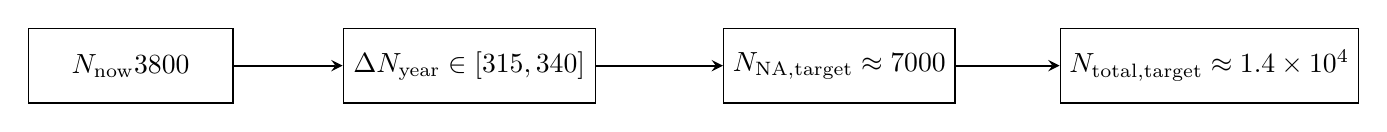
\begin{tikzpicture}[>=stealth]
\node[draw, rectangle, minimum width=2.6cm, minimum height=0.95cm] (a) at (0,0) {\(N_{\mathrm{now}}\gtrsim 3800\)};
\node[draw, rectangle, minimum width=3.2cm, minimum height=0.95cm] (b) at (4.3,0) {\(\Delta N_{\mathrm{year}}\in[315,340]\)};
\node[draw, rectangle, minimum width=2.8cm, minimum height=0.95cm] (c) at (9.0,0) {\(N_{\mathrm{NA,target}}\approx 7000\)};
\node[draw, rectangle, minimum width=3.1cm, minimum height=0.95cm] (d) at (13.7,0) {\(N_{\mathrm{total,target}}\approx 1.4\times 10^4\)};

\draw[->, thick] (a) -- (b);
\draw[->, thick] (b) -- (c);
\draw[->, thick] (c) -- (d);
\end{tikzpicture}
\caption{Transcript-derived scale ladder for Chipotle. The lecture's final case is the most numerically coherent because it ties present size, annual additions, and long-run target into one sequence.}
\end{figure}

The next question is why there is no franchising. Here the lecture's answer is extraordinarily clean. Franchising is often a way to cope with scale limits or capital needs. But at Chipotle the balance sheet is described as a fortress:
\begin{equation}
C_{\mathrm{cash}}\gtrsim \$2\times 10^9, \qquad D_{\mathrm{debt}}=0.
\end{equation}
That single pair of numbers explains why control can be preserved. If capital is abundant and debt is absent, external franchise partners are not needed to fund growth.

\begin{figure}
\centering
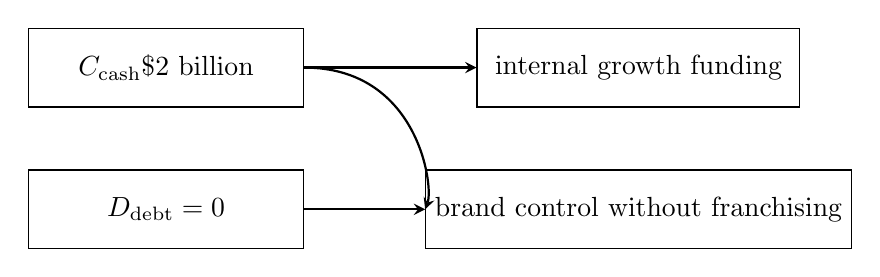
\begin{tikzpicture}[>=stealth]
\node[draw, rectangle, minimum width=3.5cm, minimum height=1.0cm] (cash) at (0,0.9) {\(C_{\mathrm{cash}}\gtrsim \$2\) billion};
\node[draw, rectangle, minimum width=3.5cm, minimum height=1.0cm] (debt) at (0,-0.9) {\(D_{\mathrm{debt}}=0\)};
\node[draw, rectangle, minimum width=4.1cm, minimum height=1.0cm] (growth) at (6,0.9) {internal growth funding};
\node[draw, rectangle, minimum width=4.1cm, minimum height=1.0cm] (control) at (6,-0.9) {brand control without franchising};

\draw[->, thick] (cash) -- (growth);
\draw[->, thick] (debt) -- (control);
\draw[->, thick] (cash.east) .. controls (3.2,0.9) and (3.4,-0.6) .. (control.west);
\end{tikzpicture}
\caption{Transcript-derived fortress balance sheet schematic. The lecture links cash abundance and zero debt directly to internal control of the expansion process.}
\end{figure}

The interview then sharpens into its cleanest portable doctrine: responsibility and accountability are not the same thing.

\begin{definition}
For a task \(T\), let \(\mathcal R(T)\) be the set of people responsible for contributing to it, and let \(a(T)\) be the designated accountable owner of the outcome, when such an owner exists.
\end{definition}

The lecture's management logic is then
\begin{equation}
|\mathcal R(T)|>1,\qquad a(T)=\varnothing
\quad \Longrightarrow \quad
\text{shared responsibility but no true accountability.}
\end{equation}
That is as sharp a statement as anything in the episode. Many may work on a task; one must own its completion.

\begin{figure}
\centering
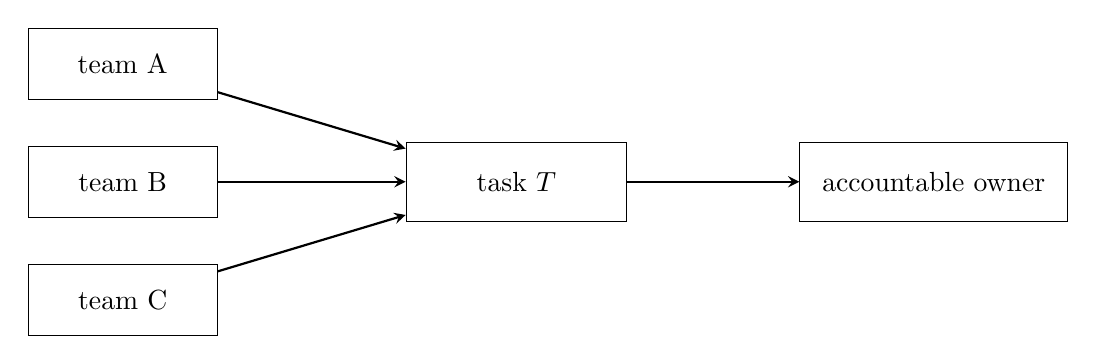
\begin{tikzpicture}[>=stealth]
\node[draw, rectangle, minimum width=2.4cm, minimum height=0.9cm] (r1) at (0,1.5) {team A};
\node[draw, rectangle, minimum width=2.4cm, minimum height=0.9cm] (r2) at (0,0) {team B};
\node[draw, rectangle, minimum width=2.4cm, minimum height=0.9cm] (r3) at (0,-1.5) {team C};

\node[draw, rectangle, minimum width=2.8cm, minimum height=1.0cm] (t) at (5,0) {task \(T\)};
\node[draw, rectangle, minimum width=3.4cm, minimum height=1.0cm] (a) at (10.3,0) {accountable owner};

\draw[->, thick] (r1) -- (t);
\draw[->, thick] (r2) -- (t);
\draw[->, thick] (r3) -- (t);
\draw[->, thick] (t) -- (a);
\end{tikzpicture}
\caption{Responsibility may be distributed, but accountability must terminate in one owner. The lecture presents this as a practical operational rule, not merely as management jargon.}
\end{figure}

The final move in the episode is easy to miss if we read too quickly. The Chipotle speaker says one cannot save one's way to prosperity and recommends investment in consumer experience and team-member experience:
\begin{equation}
I_{\mathrm{consumer}} + I_{\mathrm{team}} \longrightarrow \text{outsized future dividends}.
\end{equation}
This does not cancel the gel-nails founder's frugality lesson. It refines it. Wasteful spending and strategic investment are not the same act. Early in the lecture, money is saved from status leakage; late in the lecture, money is deployed into the machine where it can improve the product, the team, and the future return stream.

\subsection{Question \& Answer}

\paragraph{Question.} Why refuse franchising when the demand is already this large?

\paragraph{Answer.} Because franchising solves a particular problem, and the lecture suggests that Chipotle does not currently have that problem. If a company lacks capital or lacks the ability to manage scale directly, franchising can distribute the burden. But if
\[
C_{\mathrm{cash}}\gtrsim \$2\times 10^9, \qquad D_{\mathrm{debt}}=0,
\]
then expansion can be financed internally, and control over brand execution can remain centralized. The refusal to franchise is therefore not anti-growth. It is a claim that growth need not be purchased by giving away operational authority.

\section{Summary}

By the end of the lecture the opening spectacle has been translated into a set of mechanisms. We have moved from visible objects to hidden structure: invention with unusually strong unit economics, reinvestment without debt, value capture at the transaction junction, delegation and leverage under pressure, access sold as a scarcity product, professional income turning toward industrial ownership, and corporate scale secured by a fortress balance sheet and a hard distinction between responsibility and accountability.

The lecture's achievement is not that it delivers one slogan about wealth. It is that it walks us, case by case, through several different wealth grammars while preserving the shock and rhythm of street-side discovery. The recurrent forms can be written compactly:
\[
K_{t+1}=K_t+\Pi_t-W_t, \qquad
\mathcal I=\text{resource owner}\longleftrightarrow \text{dealmaker}\longleftrightarrow \text{capital / operator}, \qquad
|\mathcal R(T)|>1,\ a(T)=\varnothing.
\]
The details change from inventor to dealmaker to operator to executive, but the deeper lesson is stable. Wealth appears in different costumes; the chapter's job is to keep following the machinery underneath.